\documentclass[a4paper,11pt]{article}

% Identificação
\newcommand{\pbtitulo}{Hyperledger Fabric}
\newcommand{\pbversao}{1.0}

\usepackage{../sty/tutorial}

%----------------------------------------------------------------------
% Início do Documento
%----------------------------------------------------------------------
\begin{document}
	
\maketitle % mostrar o título
\thispagestyle{fancy} % habilitar o cabeçalho/rodapé das páginas

%--------------------------------------------------------------------------
% AGRADECIMENTOS
%--------------------------------------------------------------------------
\renewcommand{\abstractname}{Agradecimentos}
\begin{abstract}
  % O primeiro caractere deve vir com \initial{}
  \initial{A}\textbf{gradeço ao mestre Fernando Anselmo\cite{fernandoanselmo,credito, publicacaofernando} por sempre compartilhar seus conecimentos e assim motivar outras pessoas a fazerem o mesmo, e também por tornar público seus scripts LaTeX\cite{latex}, confesso que nunca tinha se quer ouvido falar sobre e agora sou totalmente adepto.}
\end{abstract}

%--------------------------------------------------------------------------
% RESUMO DO ARTIGO
%--------------------------------------------------------------------------
\renewcommand{\abstractname}{Resumo}
\begin{abstract}
  % O primeiro caractere deve vir com \initial{}
  \initial{N}\textbf{este artigo vou falar um pouco sobre essa tecnologia que vem cada vez mais ganhando atenção mundo a fora, atraindo olhares das mais renomadas empresas de tecnologia e também de desenvolvedores por toda parte do globo terrestre.}
\end{abstract}

%--------------------------------------------------------------------------
% CONTEÚDO DO ARTIGO
%--------------------------------------------------------------------------
\section{Blockchain}
Blockchain é um livro-razão (ledger) de transações imutáveis, mantido dentro de uma rede distribuída de nós pares (peers). Esses nós mantêm uma cópia do livro (ledger), aplicando transações que foram validadas por um protocolo de consenso, agrupadas em blocos que incluem um hash que liga cada bloco ao bloco anterior.

Na Figura 1, faço uma analogia com um trem para facilitar o entendimento de uma cadeia de blocos. Primeiro teremos a cabine do trem, ela será nosso bloco genesis, agora perceba que a cada estção em que o trem vai passando é adicionado um novo vagão. Cada vagão adicionado será de forma analoga um novo bloco e cada estação será a conclusão de um trabalho e assim vai formando uma cadeia onde todos os vagões ou blocos estarão interligados. 
\begin{figure}[H]
	\centering
	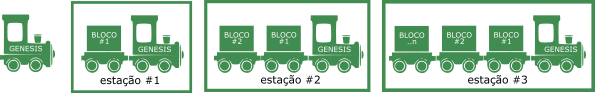
\includegraphics[width=1.0\textwidth]{imagens/conceito-blocos-trem.png}
	\caption{Exemplo de uma cadeia de blocos}
\end{figure}

\subsection{Origen do Blockchain}
\subsection{Algoritmos de Consenso}

\section{Hyperledger}
Hyperledger\cite{hyperledger} é uma comunidade de código aberto "estabelecida sob a Linux Foundation\cite{linuxfoundation}, que tem uma história longa e muito bem-sucedida de nutrir projetos de código aberto sob uma governança aberta que desenvolve comunidades sustentáveis e ecossistemas prósperos" focada no desenvolvimento de um conjunto de estruturas, ferramentas e bibliotecas para implantação de blockchain em nível corporativo.

\subsection{Hyperledger Fabric}
Hyperledger Fabric\cite{hyperledgerfabric} é uma plataforma do tipo DLT (Distributed Ledger Technologies) de código aberto de nível empresarial, projetada para uso corporativo desde o início.
\begin{figure}[H]
	\centering
	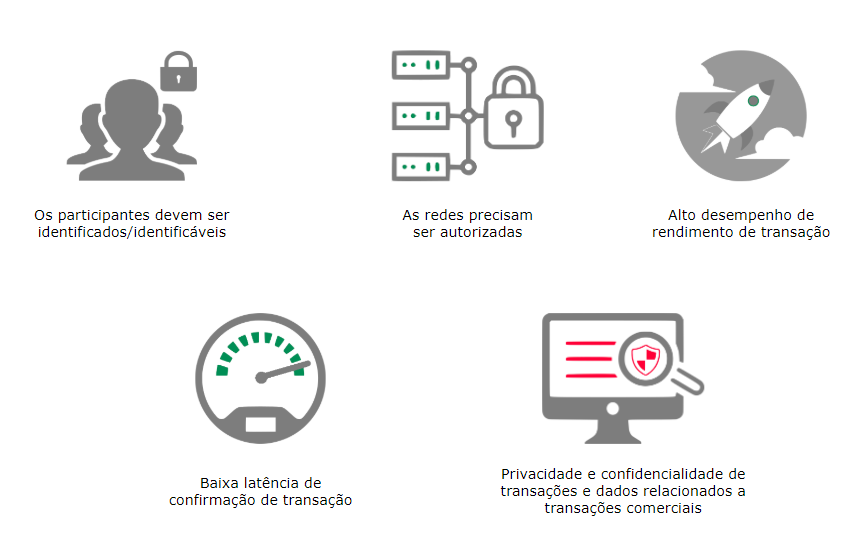
\includegraphics[width=0.9\textwidth]{imagens/requisitos.png}
	\caption{Principais requisitos para uso corporativo}
\end{figure}

\subsection{Criando sua primeira rede Blockchain}
\subsubsection{Pré-requisitos}
\subsubsection{Definindo diretório de trabalho}
\subsubsection{Baixando Imagens Hyperledger Fabric}
\subsubsection{Iniciando a rede}

\section{Conclusão}

\section{Sobre o autor}
Praticante dos princípios ágeis para desenvolvimento de software, focado na entrega de valor.

Adepto do software \textbf{Open Source} (Software Livre), estou sempre em busca de novos conhecimentos e desafios relacionados ao desenvolvimento de software que agregam valor tanto no âmbito pessoal quanto profissional. 

\begin{center}
``\underline{Livre} significa que esta apostila é gratuita e pode ser compartilhada a vontade. \underline{Open Source} além de livre todos os arquivos que permitem a geração desta (chamados de arquivos fontes) devem ser disponibilizados para que qualquer pessoa possa modificar ao seu prazer, gerar novas, complementar ou fazer o que quiser.''
por Fernando Anselmo\cite{fernandoanselmo}
\end{center}

%--------------------------------------------------------------------------
% REFERÊNCIAS
%--------------------------------------------------------------------------
\begin{thebibliography}{5}
  \bibitem{linuxfoundation} 
  The Linux Foundation \\
  \url{https://www.linuxfoundation.org/}

  \bibitem{hyperledger} 
  Hyperledger \\
  \url{https://hyperledger.org/}

  \bibitem{hyperledgerfabric} 
  Hyperledger Fabric \\
  \url{https://www.hyperledger.org/use/fabric}

  	\bibitem{latex} 
	LaTeX \\
	\url{https://latex.net/}
	
	\bibitem{credito} 
	Essa apostila utiliza scripts LaTeX\cite{latex} disponibilizados por Fernando Anselmo\cite{fernandoanselmo}  \\
	\url{https://github.com/fernandoans/publicacoes}

	\bibitem{fernandoanselmo} 
	Fernando Anselmo - Blog Oficial de Tecnologia \\
	\url{http://www.fernandoanselmo.blogspot.com.br/}

	\bibitem{publicacaofernando}
	Encontre publicações de Fernando Anselmo\cite{fernandoanselmo} em \\
	\url{https://cetrex.academia.edu/FernandoAnselmo}

	\bibitem{github} 
	Encontre essa e outras publicações minhas em \\
	\url{https://github.com/deusimarferreira/artigos}
\end{thebibliography}
  
\end{document}
